\documentclass{standalone}
\usepackage{tikz}
\usetikzlibrary{patterns, positioning}

\begin{document}
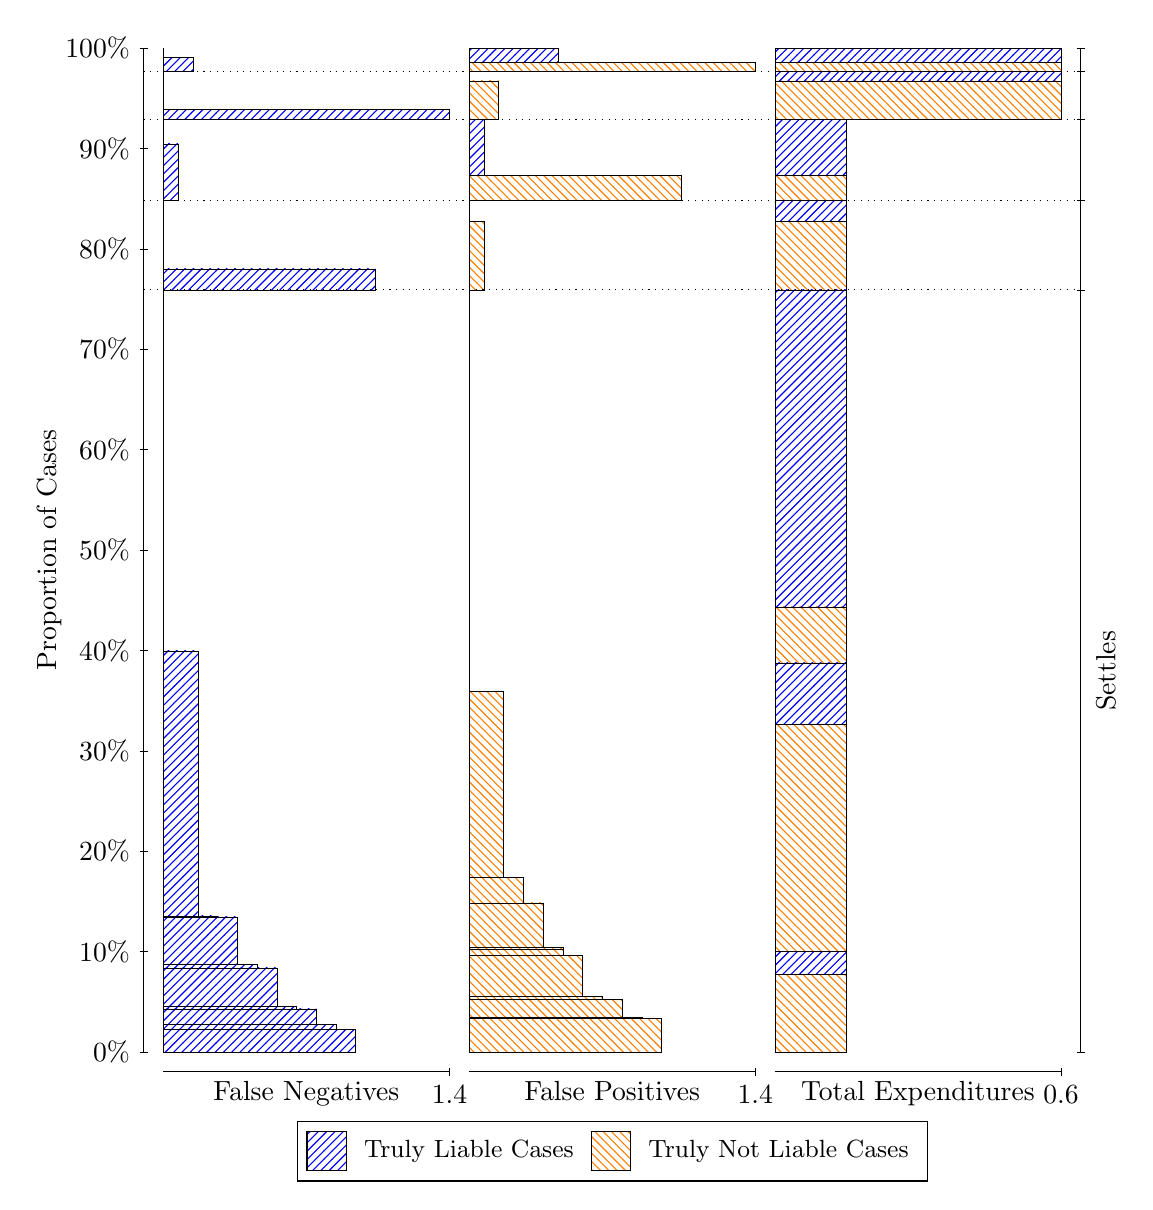
\begin{tikzpicture}
\draw[black, very thin] (1.5,1.75) -- (1.5,14.5);
\node[rotate=90, anchor=center] at (0.3, 8.125) {Proportion of Cases};
\draw[black, very thin] (1.45,1.75) -- (1.55,1.75);
\node[anchor=east] at (1.45, 1.75) {0\%};
\draw[black, very thin] (1.45,3.025) -- (1.55,3.025);
\node[anchor=east] at (1.45, 3.025) {10\%};
\draw[black, very thin] (1.45,4.3) -- (1.55,4.3);
\node[anchor=east] at (1.45, 4.3) {20\%};
\draw[black, very thin] (1.45,5.575) -- (1.55,5.575);
\node[anchor=east] at (1.45, 5.575) {30\%};
\draw[black, very thin] (1.45,6.85) -- (1.55,6.85);
\node[anchor=east] at (1.45, 6.85) {40\%};
\draw[black, very thin] (1.45,8.125) -- (1.55,8.125);
\node[anchor=east] at (1.45, 8.125) {50\%};
\draw[black, very thin] (1.45,9.4) -- (1.55,9.4);
\node[anchor=east] at (1.45, 9.4) {60\%};
\draw[black, very thin] (1.45,10.675) -- (1.55,10.675);
\node[anchor=east] at (1.45, 10.675) {70\%};
\draw[black, very thin] (1.45,11.95) -- (1.55,11.95);
\node[anchor=east] at (1.45, 11.95) {80\%};
\draw[black, very thin] (1.45,13.225) -- (1.55,13.225);
\node[anchor=east] at (1.45, 13.225) {90\%};
\draw[black, very thin] (1.45,14.5) -- (1.55,14.5);
\node[anchor=east] at (1.45, 14.5) {100\%};

\draw[black, very thin] (13.4,1.75) -- (13.4,14.5);
\draw[black, very thin] (13.35,1.75) -- (13.45,1.75);
\node[anchor=west] at (13.35, 1.75) {};
\draw[black, very thin] (13.35,11.429) -- (13.45,11.429);
\node[anchor=west] at (13.35, 11.429) {};
\draw[black, very thin] (13.35,12.566) -- (13.45,12.566);
\node[anchor=west] at (13.35, 12.566) {};
\draw[black, very thin] (13.35,13.596) -- (13.45,13.596);
\node[anchor=west] at (13.35, 13.596) {};
\draw[black, very thin] (13.35,14.204) -- (13.45,14.204);
\node[anchor=west] at (13.35, 14.204) {};
\draw[black, very thin] (13.35,14.5) -- (13.45,14.5);
\node[anchor=west] at (13.35, 14.5) {};

\draw[black, very thin, pattern color=blue, pattern=north east lines] (1.75,1.75) rectangle (4.1931,2.0417);
\draw[black, very thin, pattern color=blue, pattern=north east lines] (1.75,2.0417) rectangle (3.9425,2.0976);
\draw[black, very thin, pattern color=blue, pattern=north east lines] (1.75,2.0976) rectangle (3.692,2.2962);
\draw[black, very thin, pattern color=blue, pattern=north east lines] (1.75,2.2962) rectangle (3.4414,2.328);
\draw[black, very thin, pattern color=blue, pattern=north east lines] (1.75,2.328) rectangle (3.1908,2.8179);
\draw[black, very thin, pattern color=blue, pattern=north east lines] (1.75,2.8179) rectangle (2.9402,2.8606);
\draw[black, very thin, pattern color=blue, pattern=north east lines] (1.75,2.8606) rectangle (2.6897,3.4665);
\draw[black, very thin, pattern color=blue, pattern=north east lines] (1.75,3.4665) rectangle (2.4391,3.4791);
\draw[black, very thin, pattern color=blue, pattern=north east lines] (1.75,3.4791) rectangle (2.1885,6.8451);
\draw[black, very thin, pattern color=orange, pattern=north west lines] (1.75,6.8451) rectangle (1.75,11.429);
\draw[black, very thin, pattern color=blue, pattern=north east lines] (1.75,11.429) rectangle (4.4437,11.695);
\draw[black, very thin, pattern color=orange, pattern=north west lines] (1.75,11.695) rectangle (1.75,12.566);
\draw[black, very thin, pattern color=blue, pattern=north east lines] (1.75,12.566) rectangle (1.9379,13.283);
\draw[black, very thin, pattern color=orange, pattern=north west lines] (1.75,13.283) rectangle (1.75,13.596);
\draw[black, very thin, pattern color=blue, pattern=north east lines] (1.75,13.596) rectangle (5.3833,13.716);
\draw[black, very thin, pattern color=orange, pattern=north west lines] (1.75,13.716) rectangle (1.75,14.204);
\draw[black, very thin, pattern color=blue, pattern=north east lines] (1.75,14.204) rectangle (2.1259,14.382);
\draw[black, very thin, pattern color=orange, pattern=north west lines] (1.75,14.382) rectangle (1.75,14.5);
\draw[black, very thin, pattern color=orange, pattern=north west lines] (5.6333,1.75) rectangle (8.0764,2.1813);
\draw[black, very thin, pattern color=orange, pattern=north west lines] (5.6333,2.1813) rectangle (7.8259,2.1897);
\draw[black, very thin, pattern color=orange, pattern=north west lines] (5.6333,2.1897) rectangle (7.5753,2.4177);
\draw[black, very thin, pattern color=orange, pattern=north west lines] (5.6333,2.4177) rectangle (7.3247,2.4603);
\draw[black, very thin, pattern color=orange, pattern=north west lines] (5.6333,2.4603) rectangle (7.0741,2.9789);
\draw[black, very thin, pattern color=orange, pattern=north west lines] (5.6333,2.9789) rectangle (6.8236,3.0484);
\draw[black, very thin, pattern color=orange, pattern=north west lines] (5.6333,3.0484) rectangle (6.8236,3.0738);
\draw[black, very thin, pattern color=orange, pattern=north west lines] (5.6333,3.0738) rectangle (6.573,3.6431);
\draw[black, very thin, pattern color=orange, pattern=north west lines] (5.6333,3.6431) rectangle (6.3224,3.968);
\draw[black, very thin, pattern color=orange, pattern=north west lines] (5.6333,3.968) rectangle (6.0718,6.3339);
\draw[black, very thin, pattern color=blue, pattern=north east lines] (5.6333,6.3339) rectangle (5.6333,11.429);
\draw[black, very thin, pattern color=orange, pattern=north west lines] (5.6333,11.429) rectangle (5.8213,12.301);
\draw[black, very thin, pattern color=blue, pattern=north east lines] (5.6333,12.301) rectangle (5.6333,12.566);
\draw[black, very thin, pattern color=orange, pattern=north west lines] (5.6333,12.566) rectangle (8.327,12.879);
\draw[black, very thin, pattern color=blue, pattern=north east lines] (5.6333,12.879) rectangle (5.8213,13.596);
\draw[black, very thin, pattern color=orange, pattern=north west lines] (5.6333,13.596) rectangle (6.0092,14.084);
\draw[black, very thin, pattern color=blue, pattern=north east lines] (5.6333,14.084) rectangle (5.6333,14.204);
\draw[black, very thin, pattern color=orange, pattern=north west lines] (5.6333,14.204) rectangle (9.2667,14.322);
\draw[black, very thin, pattern color=blue, pattern=north east lines] (5.6333,14.322) rectangle (6.7609,14.5);
\draw[black, very thin, pattern color=orange, pattern=north west lines] (9.5167,1.75) rectangle (10.425,2.7391);
\draw[black, very thin, pattern color=blue, pattern=north east lines] (9.5167,2.7391) rectangle (10.425,3.0254);
\draw[black, very thin, pattern color=orange, pattern=north west lines] (9.5167,3.0254) rectangle (10.425,5.9099);
\draw[black, very thin, pattern color=blue, pattern=north east lines] (9.5167,5.9099) rectangle (10.425,6.6915);
\draw[black, very thin, pattern color=orange, pattern=north west lines] (9.5167,6.6915) rectangle (10.425,7.4019);
\draw[black, very thin, pattern color=blue, pattern=north east lines] (9.5167,7.4019) rectangle (10.425,11.429);
\draw[black, very thin, pattern color=orange, pattern=north west lines] (9.5167,11.429) rectangle (10.425,12.301);
\draw[black, very thin, pattern color=blue, pattern=north east lines] (9.5167,12.301) rectangle (10.425,12.566);
\draw[black, very thin, pattern color=orange, pattern=north west lines] (9.5167,12.566) rectangle (10.425,12.879);
\draw[black, very thin, pattern color=blue, pattern=north east lines] (9.5167,12.879) rectangle (10.425,13.596);
\draw[black, very thin, pattern color=orange, pattern=north west lines] (9.5167,13.596) rectangle (13.15,14.084);
\draw[black, very thin, pattern color=blue, pattern=north east lines] (9.5167,14.084) rectangle (13.15,14.204);
\draw[black, very thin, pattern color=orange, pattern=north west lines] (9.5167,14.204) rectangle (13.15,14.322);
\draw[black, very thin, pattern color=blue, pattern=north east lines] (9.5167,14.322) rectangle (13.15,14.5);
\draw[black, dotted] (1.5,11.429) -- (13.4,11.429);
\draw[black, dotted] (1.5,12.566) -- (13.4,12.566);
\draw[black, dotted] (1.5,13.596) -- (13.4,13.596);
\draw[black, dotted] (1.5,14.204) -- (13.4,14.204);
\draw[black, very thin] (1.75,1.5) -- (5.3833,1.5);
\node[anchor=north] at (3.5667, 1.5) {False Negatives};
\draw[black, very thin] (5.3833,1.45) -- (5.3833,1.55);
\node[anchor=north] at (5.3833, 1.45) {1.4};

\draw[black, very thin] (5.6333,1.5) -- (9.2667,1.5);
\node[anchor=north] at (7.45, 1.5) {False Positives};
\draw[black, very thin] (9.2667,1.45) -- (9.2667,1.55);
\node[anchor=north] at (9.2667, 1.45) {1.4};

\draw[black, very thin] (9.5167,1.5) -- (13.15,1.5);
\node[anchor=north] at (11.333, 1.5) {Total Expenditures};
\draw[black, very thin] (13.15,1.45) -- (13.15,1.55);
\node[anchor=north] at (13.15, 1.45) {0.6};

\node[black, centered, rotate=90] at (13.72, 6.5895) {Settles};





\draw (7.449999999999999,1.5) node[draw=none] (baseCoordinate) {};
\begin{scope}[align=center]
        \matrix[scale=0.5, draw=black, below=0.5cm of baseCoordinate, nodes={draw}, column sep=0.1cm]{
            \node[rectangle, draw, minimum width=0.5cm, minimum height=0.5cm, pattern=north east lines, pattern color=blue] {}; &
            \node[draw=none, font=\small] (B) {Truly Liable Cases}; &
            \node[rectangle, draw, minimum width=0.5cm, minimum height=0.5cm, pattern=north west lines, pattern color=orange] {}; &
            \node[draw=none, font=\small] (B) {Truly Not Liable Cases}; \\
            };
\end{scope}

\end{tikzpicture}
\end{document}